\documentclass{article}

% Language setting
\usepackage[english]{babel}

% Set page size and margins
\usepackage[a4paper,top=2cm,bottom=2cm,left=3cm,right=3cm,marginparwidth=1.75cm]{geometry}
%

% Useful packages
\usepackage{amsmath}
\usepackage{graphicx}
\usepackage[colorlinks=true, allcolors=blue]{hyperref}

\usepackage{csquotes}% Recommended (harvard style)

\usepackage[style=authoryear-ibid,backend=biber]{biblatex}%harvard style

\graphicspath{{./images/}}

\addbibresource{books.bib}% Syntax for version >= 1.2

\title{Derive Newton's Law of Universal Gravitation from Kepler's Laws}
\author{Zhicheng Gong}
\date{December 2023}

\begin{document}
\maketitle


\section{Introduction}

The high point of the Scientific Revolution was marked by Isaac Newton's discovery of the law of universal gravitation. According to this principle, all objects exert a force on each other, directly proportional to the product of their masses and inversely proportional to the square of their distance from each other. By unifying the fundamental physical phenomena of the observable universe under a single mathematical law, Newton demonstrated the essential unity of terrestrial and celestial physics. This innovative concept of universal gravitation not only unveiled the profound significance of Johannes Kepler's three laws of planetary motion but also provided solutions to long-standing problems. It addressed the origin of tides and explained Galileo's puzzling observation that the descent of a free-falling object is independent of its weight. In achieving this, Newton realized  Kepler's goal of developing a physics based on causes \autocite{Cohen1981}.

From Tycho Brahe's experimental observations to Kepler's empirical rules, from empirical rule to a single neat and tidy equation describing the interactions, Newton generalised it to eventually reach one of the most versatile and concise laws governing every single particle in the universe. By reproducing this reasoning process, with modern mechanics explanations and intuitive geometric interpretations, this article attempts to provide a glimpse of the path to truth through a chink in the history of science.

\section{What Kepler's Second Law indicates}

Kepler's Second Law of planetary motion states that:
The radius vector to a planet sweeps out area at a rate that is independent of its position in the orbit \autocite{Morin2008}.
\[\frac{dA}{dt} = \text{Constant}\]
\subsection{Modern Approach}
During a small amount of time $dt$, the distance $\boldsymbol{r}$ of a planet from the Sun can be considered as a constant. The area swept in this case is approximately a triangle with a base of the displacement normal to the distance $V_\tau \cdot dt$ and height of the distance $r$ from the central object. 
\[dA = \frac{1}{2}\ V_\tau\ dt\cdot r\]
Or otherwise, we can use the cross product of two vectors:
\begin{align*}
    \label{eq:1}
    2\frac{dA}{dt}  = r^2 \dot{\theta} = \ \boldsymbol{r} \times \boldsymbol{v} = \ell
\end{align*}
and $\ell$ is a constant. Thus
\begin{align*}
    \frac{dA}{dt}\cdot m & =  \frac{1}{2}\boldsymbol{r} \times (\boldsymbol{v} \cdot m) 
    \\ & = \frac{1}{2}\boldsymbol{r} \times \boldsymbol{p} 
    \\ & = \frac{1}{2} \boldsymbol{L} = \text{Another constant}
    \\ & \text{ (bold symbol indicates it is a vector)}
\end{align*}
Since the area $A$ per unit time is conserved, the angular momentum $\boldsymbol{L}$ in Newtonian mechanics is a constant. 
By definition,
\begin{align*}
    \frac{d\boldsymbol{L}}{dt} & = \frac{d}{dt} (\boldsymbol{r} \times \boldsymbol{p})
    \\ &  = \frac{d\boldsymbol{r}}{dt} \times \boldsymbol{p} + \boldsymbol{r} \times \frac{d\boldsymbol{p}}{dt} 
    \\ & = \boldsymbol{v} \times (m\boldsymbol{v}) + \boldsymbol{r} \times \boldsymbol{F} 
    \\ & = 0
\end{align*}
because the cross product of two parallel vectors is zero, $\boldsymbol{r} \times \boldsymbol{F}$ is zero. So the gravitational force $\boldsymbol{F}$ is parallel to the position vector $\boldsymbol{r}$, which by definition, means that the gravity is a central force\autocite{Morin2008}. 

For us probably it makes perfect sense that gravitational forces point radially, otherwise it would break the rotational symmetry. However, since we would like to get to Newton's law of universal gravitation from scratch, it worth proving.

\subsection{Newton's original approach}

In Newton's very first proposition of the \textit{Principia}, he considers a particle moving along a straight line at a uniform velocity. The particle moves equal distances in equally distributed time intervals. A point F is chosen at a certain distance h above the line. The triangles formed by connecting F to any of the intervals obviously all have the same area as shown in figure \ref{fig:polygon}.
\[S_{\Delta ABF} = S_{\Delta BCF}\]
Then in a different scenario, the body initially moves as before with a constant velocity. At the end of the second interval it experiences an impulse along the line connecting the point F. It is not hard to show that the new third triangle still has the same area as the previous two.
\[S_{\Delta BC^{\prime} F} = S_{\Delta BCF} = S_{\Delta ABF}\]
Similarly, at the end of the third and all the following intervals, the particle will be given an impulsive towards point F. All the triangles have the same area as the previous ones thus the polygonal path obeys the law of areas. In the limiting cases the  time intervals approach zero, thus the impulses now form a continuous centre force pointing to the chosen focus F. In this way, Newton got to the same argument that a central force generates a curve obeying the law of areas. And vice versa motion in a curve described by the law of areas implies a central force and the conservation of angular momentum \autocite{Cohen1981}.

\begin{figure}[ht]
    \centering
    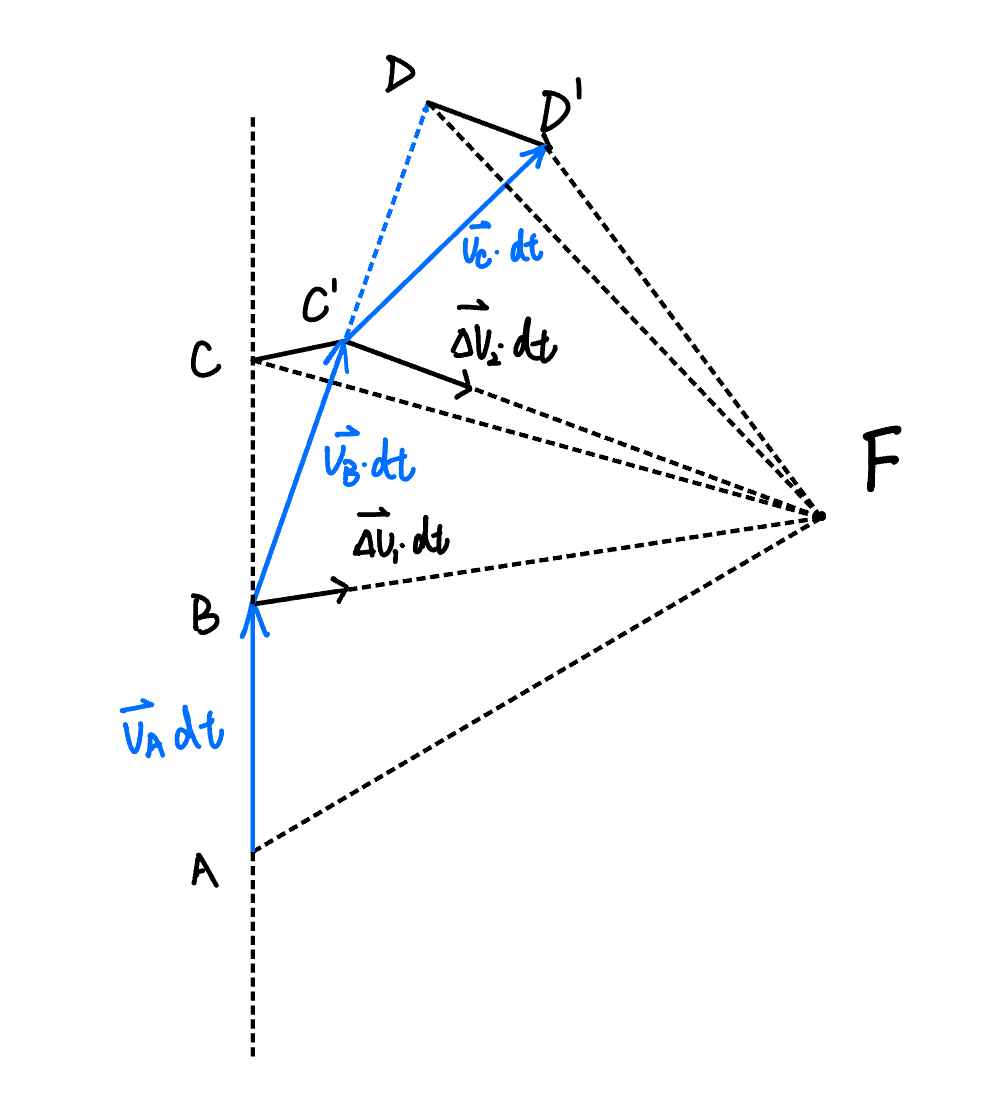
\includegraphics[width=0.5\linewidth]{images/IMG_6728.PNG}
    %\caption{Caption}
    \label{fig:polygon}
\end{figure}

\section{What Kepler's First Law indicates}

\subsection{An Approximation}

In high school level mechanics, trajectories are considered to be perfect circles as stated by Nicolaus Copernicus's heliocentric theory, which is somewhat precise enough. The eccentricity (a dimensionless parameter measuring the amount by which its orbit deviates from a perfect circle) of the Earth's orbit is currently about 0.0167 (a perfect circle is 0); its orbit is nearly circular. Venus and Neptune have even lower eccentricities. In this case planets make uniform circular motion. Gravity provides centripetal force, \footnote{In 1680 Robert Hooke introduced Newton to a new way of analyzing motions in two components, an inertia component and a centripetal component. It worth mention that it took quite a while for Newton to realize the importance of considering centripetal acceleration pointing to the pivot rather than the older and misleading notion of an imaginary centrifugal force, a force cannot be traced to the interaction of physical objects, which somehow exerts on rotating particles out of  nowhere\autocite{Cohen1981}.}
\[F = m \left( \frac{2\pi}{T} \right) ^ 2 r \Longrightarrow F \propto \frac{r}{T ^ 2} \]
in which $T$ is the period of circular motion, $m$ is the mass of the planet and $r$ is the radius of circular trajectories. From the Third Law of  $T ^ 2 \propto r ^ 3$. This gives
\[F \propto r^{-2} \]
the inversely proportional law - the core of the  Law of Universal Gravitation. Several people besides Newton were closely associated with this problem including Robert Hooke \autocite{French1971}.




\subsection{Generalized situation}

To be more accurate and generalized, the Kepler's First law modified the heliocentric theory, replacing its circular orbits with elliptical trajectories with the Sun at one of the two focuses.

The proof that ellipses rather than circles, are also explained by the inverse-square law of force, was the product of Newton's genius alone\autocite{French1971}.

In polar coordinates $r$ and $\theta$ centred at one of the focus :

\[r = \frac{P}{1 - e\cos{\theta}} = \frac{a(1 - e^2)}{1 - e\cos{\theta}}\]
or
\[u = \frac{1}{r} = \frac{1}{P} - \frac{e\cos{\theta}}{P}\]
in which $P=\frac{b^2}{a}$ and $e = \frac{c}{a}$ are constants determined by the shape of the trajectories.
To prove that, we  can start with the definition of ellipses: at any point on the ellipse, the sum of the distances from the point to two focuses $ea$ apart is constant.
\[r + r^\prime = 2a\]
Squaring both sides,
\[{r^\prime} ^ 2 = 4a^2 - 4ar + r^2\]
In the triangle $FPF^\prime$ , applying the law of cosines gives
\[{r^\prime} ^ 2 = r^2 +(2ea)^2 - 4ear\cos{\theta}\]
Thus,
\[4a^2 - 4ar + r^2 = r^2 +(2ea)^2 - 4ear\cos{\theta}\]
\[r(1-e\cos{\theta}) = a(1 - e^2)\]
\[r = \frac{a(1 - e^2)}{1- e\cos{\theta}} = \frac{P}{1 - e\cos{\theta}}\]
Differentiating with respect to $\theta$ provides
\[\frac{dr}{d\theta} = \frac{ep \sin{\theta}}{(1-e \cos{\theta})^2} = \frac{r^2}{p} e \sin{\theta}\]
Retrieve the Second Law
\[\dot r = \frac{dr}{d\theta} \dot \theta = \frac{dr}{d\theta} \frac{\ell}{r^2} = \frac{\ell}{p} e \sin{\theta}\]
Now differentiate again with respect to $\theta$
\[\frac{d\dot r}{d\theta} = \frac{\ell}{p} e \cos{\theta}.\]
\begin{equation*}
    \ddot r = \frac{d \dot r}{d \theta} \dot \theta = \frac{\ell^2}{ r^2 p} e\cos{\theta} = \frac{\ell^2}{r^2 p} \left( \frac{p}{r}-1 \right) = \frac{\ell^2}{r^2} \left( \frac{1}{r}-\frac{1}{p}\right)
    \label{r double dot}
\end{equation*}
    
\subsection{Kinematics in polar coordinate}
In polar coordinates, two scalar variables are used to mark a position, $r$ and $\theta$, or we can replace the distance and bearing with a vector $\boldsymbol{r} = r\cdot \boldsymbol{e_r}$ (bold symbol indicates it is a vector and $\boldsymbol{e_r}$ is a unit vector).
\begin{figure}
    \centering
    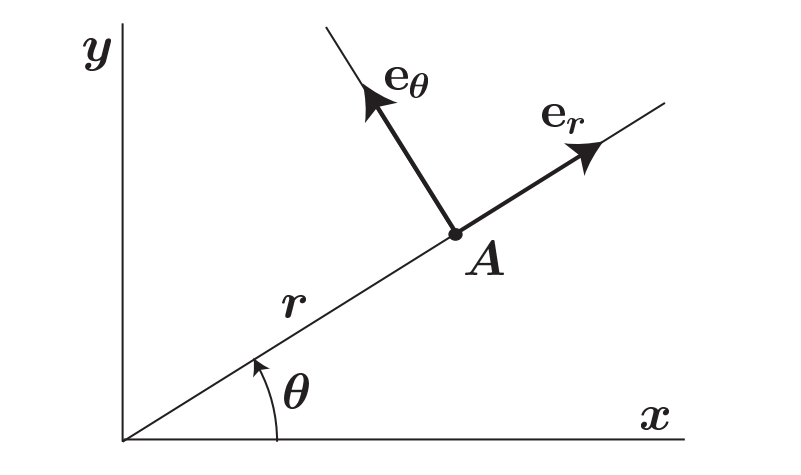
\includegraphics[width=0.5\linewidth]{images/polar_coordinate.png}
    \caption{Polar Coordinate\autocite{Widnall2008}}
    \label{fig:PolarCoor}
\end{figure}
Since $\boldsymbol{r}$ and the unit vector are obviously changing with respect to time, in polar coordinate we have 
\[\frac{d\boldsymbol{e_r}}{d\theta} = \boldsymbol{e_\theta}, \space \frac{d\boldsymbol{e_\theta}}{d\theta} = -\boldsymbol{e_r}.\]
Multiplying these expressions by $\frac{d\theta}{dt} \equiv \dot\theta$,  we obtain
\[\frac{d \boldsymbol{e_r}}{d \theta} \frac{d \theta}{d t} \equiv \frac{d \boldsymbol{e_r}}{d t}=\dot{\theta} \boldsymbol{e_\theta}, \text { and }  \frac{d \boldsymbol{e_\theta}}{d t}=-\dot{\theta} \boldsymbol{e_r}.\]
Differentiate $\boldsymbol{r}$ with respect to time gives
\[\boldsymbol{v} = \dot{\boldsymbol{r}} = \dot{r} e_r + r\dot{e_r} = \dot{r} e_r + r \dot\theta e_\theta.\]
Differentiate again with respect to time, we obtain the acceleration
$$
\boldsymbol{a}=\dot{\boldsymbol{v}}=\ddot{r} \boldsymbol{e}_{r}+\dot{r} \dot{\boldsymbol{e}}_{r}+\dot{r} \dot{\theta} \boldsymbol{e}_{\theta}+r \ddot{\theta} \boldsymbol{e}_{\theta}+r \dot{\theta} \dot{\boldsymbol{e}}_{\theta}
$$
which is
$$
\boldsymbol{a}=(\ddot{r}-r \dot{\theta}^{2}) \boldsymbol{e}_{r}+(r \ddot{\theta}+2 \dot{r} \dot{\theta}) \boldsymbol{e}_{\theta}.
$$
It worth mention that the first two terms, $a_{r}=\left(\ddot{r}-r \dot{\theta}^{2}\right)$ is the radial acceleration component, and the tangential acceleration component $a_{\theta}$ has two terms in which $2 \dot{r} \dot{\theta}$ is called Coriolis acceleration. 

\subsection{Inverse-square Law}

Rewrite $\boldsymbol{a}$ to be
\begin{align*}
    \boldsymbol{a} & =(\ddot{r}-r \dot{\theta}^{2}) \boldsymbol{e}_{r}+\frac{1}{r} \frac{d}{dt} \left( r^2 \dot\theta \right) \boldsymbol{e}_{\theta}
\\ & = (\ddot r - \frac{\ell^2}{r^3}) \boldsymbol{e}_{r} + 0
\end{align*}
From the Conservation of Momentum, the tangential component of acceleration under a central force has to be zero. Invoking $\ddot r$,
\begin{equation*}
    \boldsymbol{a} = \frac{d^2 \boldsymbol{r}}{dt^2} = - \frac{\ell ^ 2}{p} \frac{\boldsymbol{e}_{r}}{r ^ 2}.
\end{equation*}
And here we have the inverse-square law - the spirit of Newton's Universal Law of Gravitation, stating that the attraction between two bodies is inversely proportion to the square of distance between them.

\subsection{Introducing Binet equation and its proof}

Or otherwise, we can introduce Binet equation to provide the central force given the shape of a trajectory on plane polar coordinates. Mathematically, 
\[F = -m \ell ^2 u^2 \left(\frac{d^2u}{d\theta^2} + u \right),\]
in which,
\[\ell = \boldsymbol{r} \times \boldsymbol{v} \text{, and } u = \frac{1}{r}.\]
The conservation of angular momentum is the only thing we need to prove Binet equation. From the radial acceleration in polar coordinates $a_{r}$ and Newton's Second Law,
\begin{equation*}
    \frac{F}{m} =\left(\ddot{r}-r \dot{\theta}^{2}\right)
\end{equation*}
Retrieve the First Law,
\[\frac{\ell}{r^2} = \dot \theta\]
\[\frac{d^2r}{dt^2} = \frac{d(\frac{dr}{dt})}{dt} = \frac{d(\frac{dr}{d\theta} \cdot \frac{d\theta}{dt})}{dt} = \frac{d(\frac{dr}{d\theta} \cdot \frac{\ell}{r^2})}{dt}\]
Define $u = \frac{1}{r}$.
\begin{align}
\ddot r & =\frac{d^2r}{dt^2} = \frac{d\left(-\frac{1}{u^2}\left(\frac{d u}{d \theta}\right) \ell u^2\right)}{d t}=\frac{d\left(-\frac{d u}{d \theta} \ell\right)}{d t} 
\\ & =-\ell \frac{d\left(\frac{d u}{d \theta}\right)}{d t}=-\ell \frac{d \theta}{d t} \frac{d\left(\frac{d u}{d \theta}\right)}{d \theta}=-\ell^2 u^2 \frac{d\left(\frac{d u}{d \theta}\right)}{d \theta}=-\ell^2 u^2 \frac{d^2 \theta}{d \theta^2}
\end{align}
Thus,
\begin{align*}
    \frac{F}{m} & = \left(\ddot{r}-r \cdot \frac{\ell ^2}{r^4}\right)
    \\ & F = -m \ell ^2 u^2 \left(\frac{d^2u}{d\theta^2} + u\right)
\end{align*}
To apply that in Kepler's Laws, deduce $\frac{d^2 u}{d\theta^2} = -\frac{e\cos{\theta}}{P}$ from the equation of ellipses and substitute it into the Binet equation provides
\begin{align*}
    F & =  -m \ell ^2 u^2 \left(\frac{d^2u}{d\theta^2} + u\right)
    \\ & = -m \ell ^2 u^2 \left( -\frac{e\cos{\theta}}{P}+\frac{1}{P} + \frac{e\cos{\theta}}{P} \right)
    \\ & = -\frac{m\ell ^2 u^2}{P} = -\frac{m}{r^2} \cdot \left( \frac{\ell^2}{P} \right)
\end{align*}
and we arrive at the same inverse-square law.

\subsection{An intuitive alternative}

In 1689, two years after the publication of the \textit{Principia}, Newton received a letter from John Locke. He said that he had trouble understanding the mathematics so he wrote to request for a less formidable explanation of the deduction of the inverse-square law from the observed elliptic orbits of the planets. Newton replied with a delightfully simple argument resting on a remarkable property of the elliptic orbits - their geometrical symmetry, which exists in spite of the fact that in kinematic and dynamic terms the orbits are asymmetrical \autocite{French1971}.

\begin{figure}[ht]
    \centering
    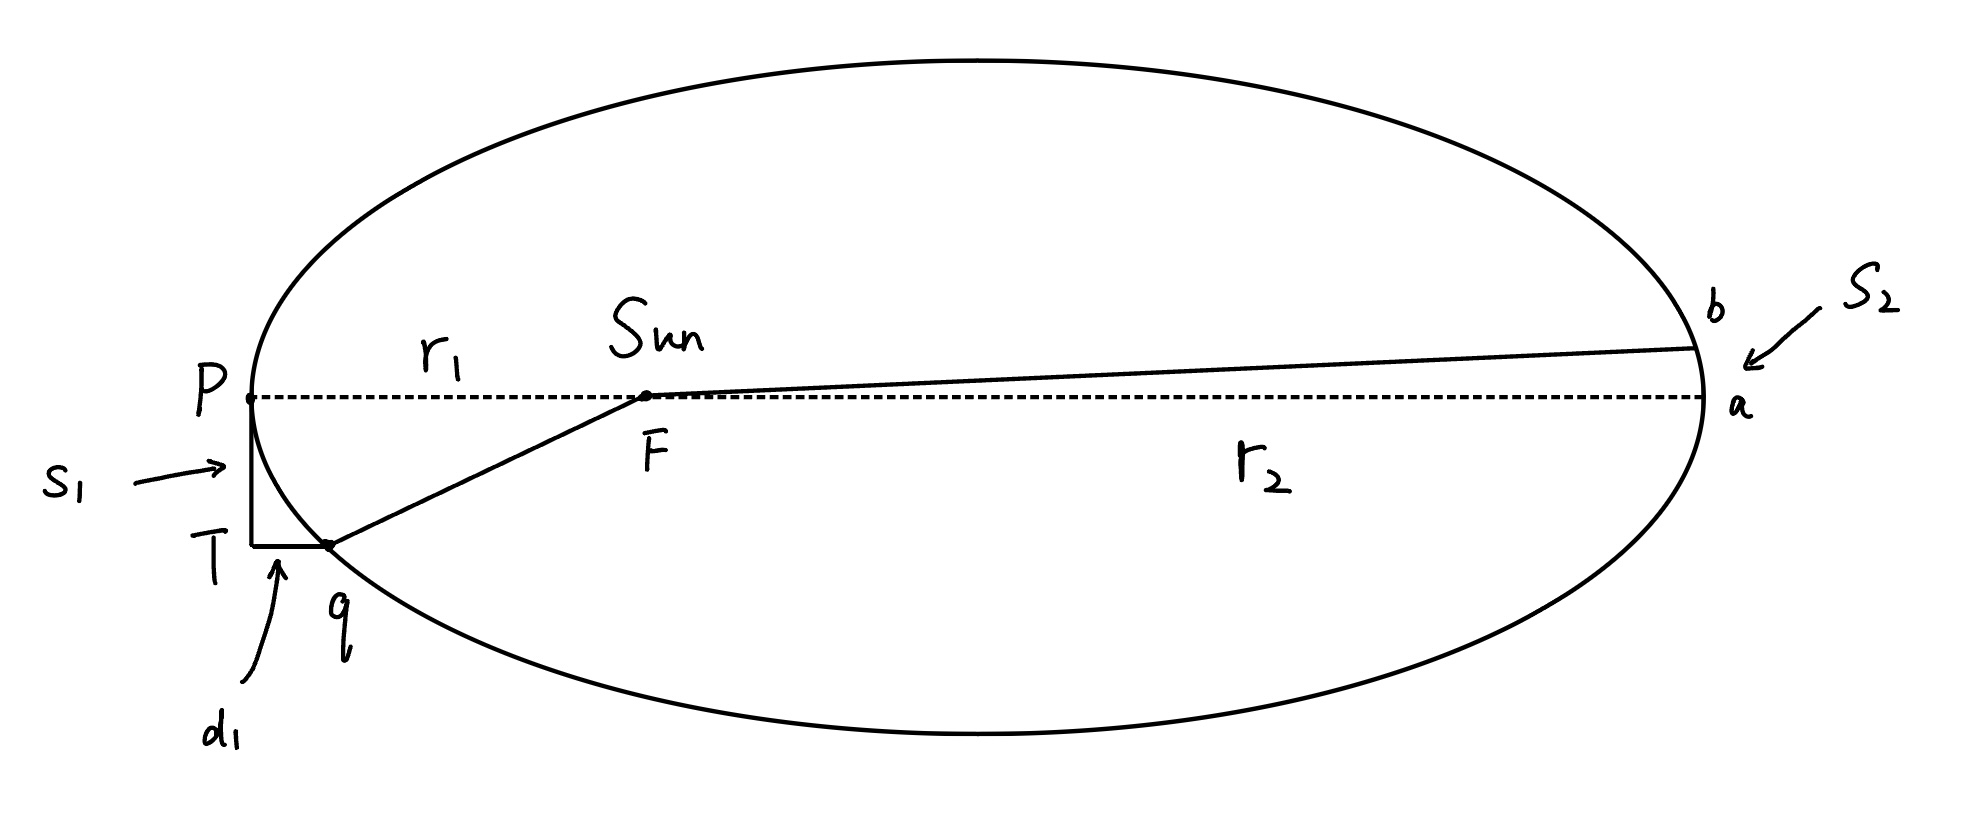
\includegraphics[width=0.5\linewidth]{images/IMG_6725.PNG}
    \label{fig:enter-label}
\end{figure}

Consider the motion of a body at the perihelion point $p$ and its aphelion point $a$ as shown in the figure. The $pq$ and $ab$ are the arcs that would be traveled in a small amount of time just after passing the two points. The lengths of arcs are related to distances from the centre body by Kepler's Second Law or the law of equal areas. Using the fact that at two points the planet's velocity is tangential to the position vector, we have
\[r_1 s_1 = r_2 s_2.\]
With the presence of gravitational force, the planet would fall through a small distance $Tq = d1$. With in a very small displacement, the curve can be seen as a parabola (assuming that the acceleration is uniform and perpendicular to the position vector within such a small area). So
\[d_1 = C s_1^2\]
where C is the constant determined by the shape of the trajectory. Notice that the curve near the aphelion $ab$ is identical to the $pq$ because of symmetry. Thus, we have
\[d_2 = C s_2^2.\]
Similarly, $s_2$ is the deviation of the path from the tangential line.
\[\frac{d_1}{d_2} = \frac{s_1^2}{s_2^2}= \frac{r_2^2}{r_1^2}\]
However, the distances fallen in equal times are proportional to the acceleration and hence to the forces, it follows that the gravitational forces acting at point $p$ and $q$ are also inversely proportional to the distances $r_1$ and $r_2$ \autocite{French1971}.

This provides an intuitive explanation by accessing the distance fallen at two special points. Similar approach can be applied at other points along the trajectory to show that $F \propto \frac{1}{r^2}$, though without the perpendicular relation between the velocity and position vector, it might be even more complicated than the algebra method mentioned previously.


\section{What Kepler's Third Law indicates}

In the book \textit{The Harmonies of the World}\autocite{kepler1619} published in 1618 by Johann Kepler, he triumphantly wrote: "I first believed I was dreaming. But it is absolutely certain and exact that the ratio which exists between the periodic times of any two planet is precisely the ratio of the $\frac{3}{2}$th powers of the mean distances."  In another word, the square of a planet's orbital period is proportional to the cube of the length of the semi-major axis of its orbit, or
\begin{equation*}
    \frac{a^3}{T^2} = \text{A constant } \epsilon
\end{equation*}

Next we would need to prove that the attraction is proportional to the mass of the central body
Invoking Kepler's First Law, $\frac{dA}{dt} = \frac{\ell}{2} = $ Constant. In a periol $T$, the area swept by the position vector is the area of the whole ellipse $\pi ab$ , so $\frac{\Delta A}{\Delta T} = \frac{\pi ab}{T}$, thus, $T = \frac{2\pi ab}{\ell}$
Substitute the period $T$ into the third law,
\begin{equation*}
    \frac{a^3}{T^2} = \frac{a\ell^2}{4\pi b^2} = \frac{1}{4\pi} \cdot (\frac{\ell^2}{P}) = \epsilon
\end{equation*}
Since $4\pi$ is a constant and $\epsilon$ depends on the central body, $\frac{\ell^2}{P}$ also depends on the central body.
\begin{align*}
    \boldsymbol{a} & =  - \frac{\ell ^ 2}{p} \frac{\boldsymbol{e}_{r}}{r ^ 2}
    \\ & = 4\pi \epsilon \cdot \frac{\boldsymbol{e}_{r}}{r ^ 2}
    \\ F & = 4\pi m \cdot \epsilon \cdot \frac{\boldsymbol{e}_{r}}{r ^ 2}
\end{align*}
Thus gravity $F$ also depends on the central body. A reasonable guess is that since it is related to the central object, it should be related to the central object's mass $M$.  We have proved that the force is inversely proportional to the distance and is related to the central body's mass $M$, but there is still one last piece of the puzzle. What exact relation does the force $F$ and the mass $M$ obey?

\section{Conclusion}

From Galileo Galilei's unexplained observation that the descent of a free-falling object is independent of its weight, in another word, the acceleration given by the Earth to the object on the ground was essentially constant, the gravitational acceleration $g$, when measured at the same location, and that, according to Newton's second law, it could be known that the force given by the Earth to the object on the ground was bound to be proportional to the object's mass, $m$. After the Moon-Earth test \autocite{French1971}, since we have found that the force given by the Earth to the Moon is the same kind of force as that given by the objects on the ground, it is natural to conjecture that the force given by the Earth to the Moon should be proportional to the Moon's mass $m$. Of course, we have already derived this conclusion.

Thinking one step further, since the earth gives the effect of encircling the moon, and the sun gives the effect of encircling the earth, is the force given by the sun to the earth the same as the force given by the earth to the moon? We have every reason to make this conclusion. Taking it a step further, would any two arbitrary stars, A and B, have this force on each other? This conjecture is logical, and leads to the conclusion that if any two stars really do have such a gravitational force on each other, then based on previous gravitational explorations of terrestrial objects, it follows that "the force from A to B is proportional to the mass of B, and the force from B to A is proportional to the mass of A". 

% Or
% \begin{align*}
%     F & \propto \frac{Mm}{r ^ 2}
% \end{align*}
% Thus, we can say
% \begin{align*}
%     F & = \frac{GMm}{r^2}
%     \\ \boldsymbol{F} & = - \frac{GMm}{r^3} \cdot \boldsymbol{r}
% \end{align*}

Over the next hundred years, people have successfully verified the correctness of this proportionality through a variety of experiments and data observations.

When Newton wrote his formula for gravitation, he made his greatest conjecture: he thought that this gravitational force would not only exist between celestial bodies and other matter, but that everything in the universe should have this effect on each other. This conjecture has a very strong insight, so that this original "from the celestial" gravity is really called "universal" gravity, and countless experiments have proved time and time again that his conjecture of "universal" is correct.

From Tycho Brahe's experimental observations to Kepler's empirical rules, from empirical rule to a single neat and tidy equation describing the interactions, Newton generalised it to eventually reach one of the most versatile and concise laws governing every single particle in the universe. By reproducing this reasoning process, with modern mechanics explanations and intuitive geometric interpretations, this article attempts to provide a glimpse of the path to truth through a chink in the history of science.

% \section{Reflection}
% Further reading about the Moon-Earth test is recommended to cover the retails that are not included in this paper. More historical events and original letters and manuscripts might be helpful to understand how Newton was confused, inspired and eventually got the propositions in the \textit{Principia} formed. In this paper, all the celestial bodies are considered point mass. To prove the equivalence of this approximation, refer to Gauss's Law.


%\subdection{Application of Gauss's Law}


\printbibliography
\end{document}